\chapter{Design and Implementation} %(approx. 10 pages)\\

\section{Program Design and Interaction Mechanisms} %TODO: Julian
* Approach to design\\
* important issues and choices and their relationships to theoretical concepts and the hardware and software platforms\\
* Did you use the GPIO module? How? In terms of interrupts and the setup in the main\\
* Did you use interrupts? How?\\ 
* Did you use multiple threads / handlers? How? Why?\\
* Did you use TI-RTOS? How?\\
%TODO: Please add some references to the documents from the bibliography and add them in the table there as well.

\section{State Machine} \label{sec:statemachine}%TODO: Hendrik
To control the program flow, state machines are a suitable approach for real-time software (Lecture 2). They allow design for multi-threaded software and real-time events can be used to cause state changes. By implementing the state machine in one task, concurrency with other parts of the software is no problem because the state machine task can sleep between iterations and change its state based on events or the result values of methods called from inside the states. Even though they can not depict time constraints in every case. Tasks which are time critical should not be implemented or called inside a specific state to ensure real-time responses.

The state machine (see Fig.\ref{fig:statemachine}) is executed in an own task inside an infinite while loop with a sleep of 10 ticks between each iteration. The execution starts in the \texttt{INIT} state. There the related method from the driver library is called to set up and initialize data structures. If the method return true as an indication that it was successful, the current state is changed to \texttt{INIT\_STATION}. Again the related function from the driver library is called, this time to ensure that the platform is in its initial position and the ejector is retracted. The functions in the driver library are all implemented as blocking functions with a return value to indicate their success in execution. After successfully returning from the method call, the state will be changed to the \texttt{CHECK\_WORKPIECE} state. In this state it will only be checked if a work piece was placed in the designated position on the platform. The switching to the next state will only be executed, if the return value indicated an available work piece.
To ensure a safe testing process the moving parts will not be activated before the state \texttt{CHECK\_SAFTEY\_BARRIER} was executed and indicated a clear working zone. The state is then changed to \texttt{MEASURE\_WORKPIECE}. This state is the most important and complex one. With the platform still remaining in the bottom position, the material and color is retrieved through a driver library function call and saved into a struct which is defined in the libraries header file. Then the platform is moved up to get the height measurement from the sensor at the top. The movement of the platform is stopped by an hardware interrupt outside of the state machine. The corresponding method will return true when the top position is reached and after a little delay a measurement is triggered. This is also saved into global variable and afterwards the method \texttt{checkWorkpiece()} is called to decide if the work piece is accepted or rejected. This decision can be made based on the data available in the struct and the height variable, but in the current implementation only the height of the work piece is relevant and the material and colour are only logged for statistic purposes. The state should change to \texttt{ACCEPT\_WORKPIECE} or \texttt{REJECT\_WORKPIECE} afterwards. In case something goes wrong when moving the platform up (which would be indicated by the return value of the \texttt{movePlattform()} method), the state is changed back to \texttt{INIT\_STATION} and the checks and measurement will be repeated.
The \texttt{ACCEPT\_WORKPIECE} state first activates the air slider and then triggers a cascade of method calls to extend the ejector, retract the ejector, move the platform down and switch the air slider off again. If one of the first three methods fail the current state is changed to \texttt{INIT\_STATION} and the air slider is turned off, otherwise the new state will be \texttt{CHECK\_WORKPIECE}. Then the next work piece can be inserted and the testing process will continue.
If the work piece is rejected after the measurements, inside the \texttt{REJECT\_WORKPIECE} state as well a cascade of method calls is executed, to move the platform down, extend the ejector and retract the ejector. In any error case we return to our initialisation state of the station or in case of success the we continue in the \texttt{CHECK\_WORKPIECE} state.

A special case is the \texttt{CALIBRATE\_SENSOR} state. After each iteration of the state machine, it is checked whether the event with the ID 04 has occurred. If this is the case, the current state is changed to start the calibration, no matter if it was changed before or would just stay the same. The event is triggered by a click on the hardware up  button next to the display. Inside the state the method to execute the calibration procedure is called, then the movement of the platform is disabled to allow the operator to remove the calibration work piece manually. After that the state machine changes to the \texttt{INIT\_STATION} state.

\begin{figure}[H]
	\begin{center}
		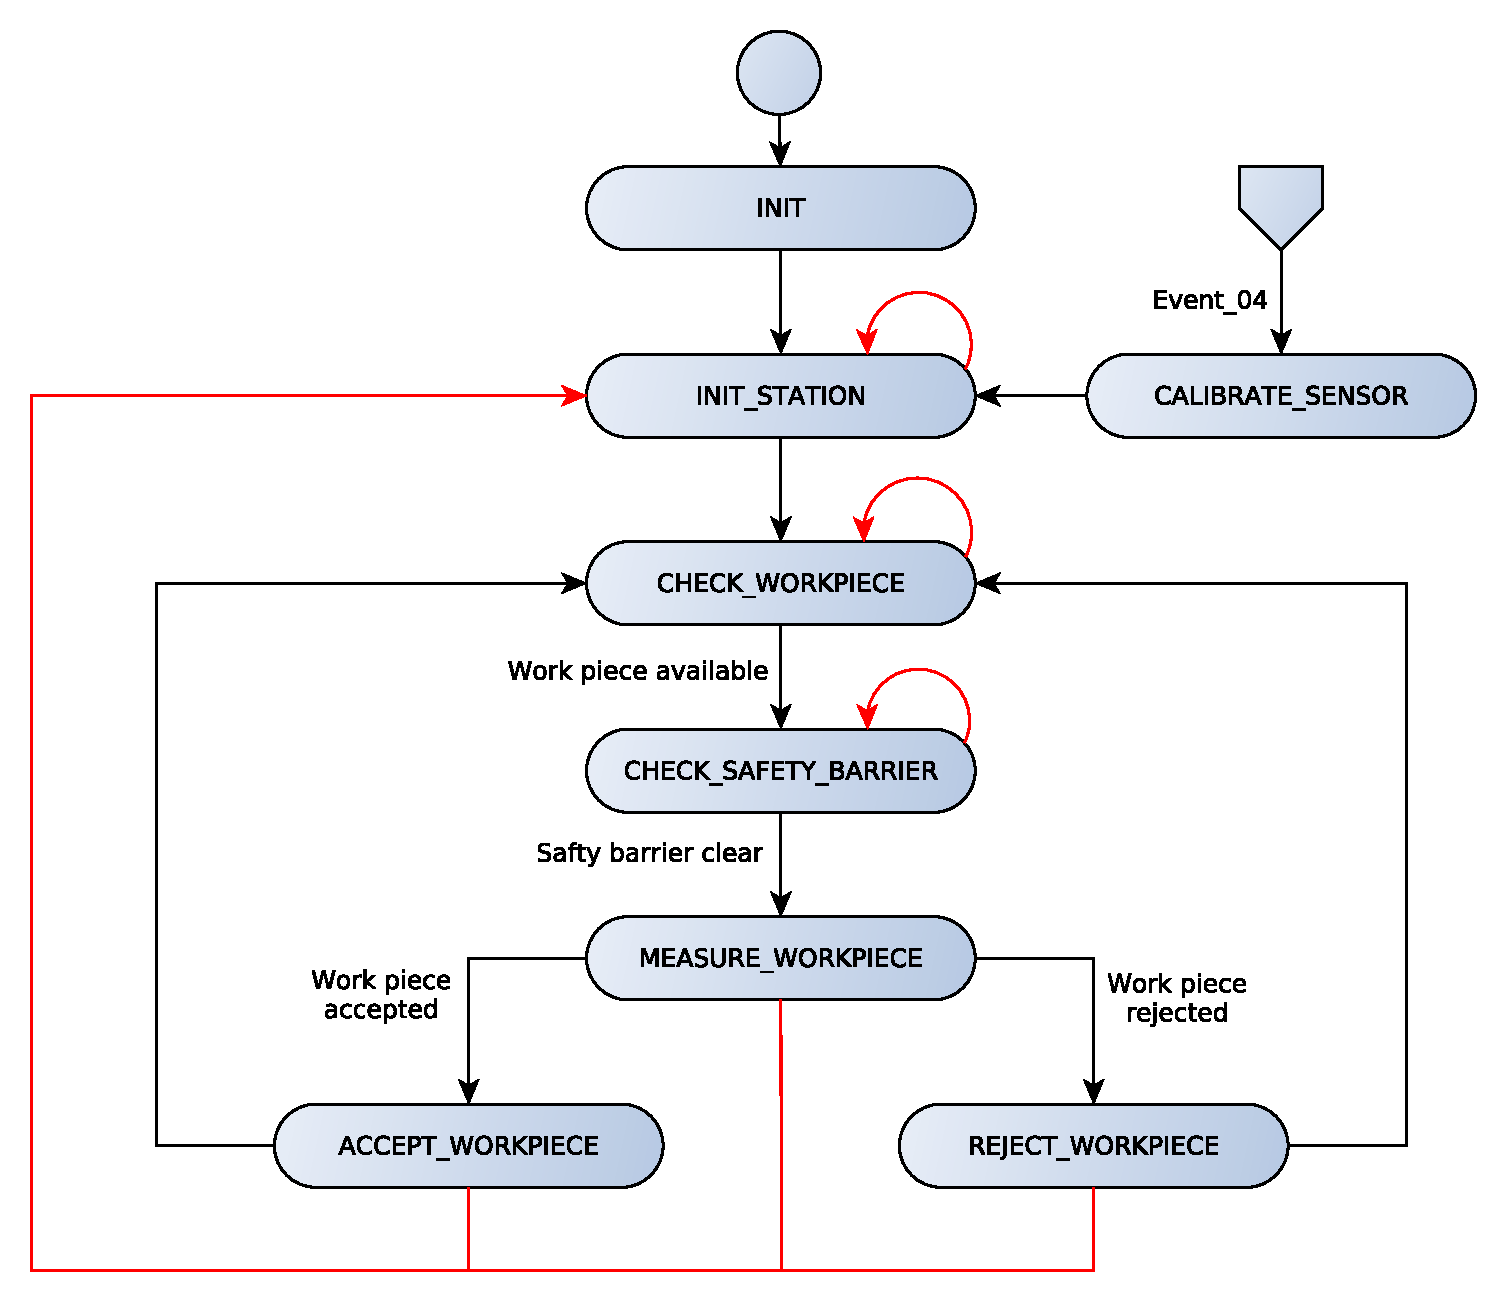
\includegraphics[scale=.60]{media/StateMachine_Main.pdf} 	
		\caption{Main State Machine}
		\label{fig:statemachine}
	\end{center}
\end{figure}

\section{Device Driver Library} \label{sec:driverlibrary} %TODO: Timo
%* Did you use the GPIO module? How? Through the qut library... Pin Map table?\\
%* Did you use the ADC? How? 

% - movement bool for disable / enable movement by user
% - material struct

The device driver library (\texttt{driverLib.h}) is providing high level functions to access the sensors and actuators of the Festo testing station. 
It uses functions of the \texttt{qut\_tiva.h}-file for pin access to the station. 
Therefore the \texttt{qut\_set\_gpio()}-function is used to change the output pins that are attached to the actuators of the station. The states of the sensors are read using the \texttt{qut\_get\_gpio()}-function. In order to get the value of the analogue height sensor a Analogue-to-Digital Converter (ADC) is used. It gets initialized by \texttt{QUT\_ADC0\_Init()} and afterwards the raw value of the sensor can be read and converted by the ADC through the \texttt{QUT\_ADC0\_Read()}-function. 

In the \texttt{driverLib.h}-file a \texttt{ColorMaterial} struct is introduced that consists of two bool-values for the attribute \glq metallic\grq and \glq black\grq. This stuct is filled with the current data of the sensors and returned by the \texttt{getMaterial()}-function of the library.\\

The library holds a bool value that is \texttt{true} as long as the movement is enabled. If this value is set to \texttt{false} the call of every function that controls one of the actuators will not perform and therefore return false since the aim cannot be reached. The value can be changed by the user or in some stages of the state machine (See Sec. \ref{sec:statemachine}). 
The function set provided by the library and their behaviours are described in the following: 

\begin{description} 
	\item[init()] In the \texttt{init()}-function the Event\_Handle and all datatypes are initialized. 
	\item[initStation()] It makes sure that the station will be in the initial position afterwards. The platform will be in lowered position and the ejector will be retracted. Other movement functions of the library are used to achieve this aim.
	\item[movePlatform(bool up, bool secureMovement)] This function moves the platform in the lowered or raised position depending on the given parameter. If the secure movement is enabled the movement of the platform will not be triggered before the security barrier is free. 
	\item[controlEjector(bool extend, bool secureMovement)] The ejector of the station will be extended or retracted depending on the given parameter. If the secure movement is enabled the movement of the ejector will not be triggered before the security barrier is free. 
	\item[controlAirSlider(bool enable)] Depending on the given bool value the air slider will be activated or deactivated.
	\item[toggleEnableMovement()] It toggles the state of the movement enable bool. If the movement is going to be disabled then all pins of the actuators are set to 0 to stop every movement of the station.
	\item[enableMovement(bool enable)] Sets the state of the movement enable bool to the given parameter value. If the movement is going to be disabled then all pins of the actuators are set to 0 to stop every movement of the station.
	\item[senseWorkpiece()] Returns if there is current a workpiece in the platform or not.
	\item[senseSafetyBarrierClear()] Returns if the safety barrier is clear or if something is in between it.
	\item[getRawWorkpieceHeight()] Returns the raw value of the ADC that is attached to the height sensor of the station. 
	\item[getWorkpieceHeight(float slope, float intersect)] Returns the height of the current workpiece in $10^{-1}$mm based on the given slope, y-intersect and the raw value of the ADC.
	\item[getMaterial()] Returns a \texttt{ColorMaterial}-struct that includes the current measurement of the color and the metallic value of the workpiece.
\end{description}

The functions are designed to be blocking until the desired movement or action is fulfilled. For example the \text{movePlatform(..)}-function waits until the platform is in the correct position and returns true afterwards. It would also be possible to design functions that just trigger a certain movement, but then another function that inspects the state of the movement has to be called by the state machine in order to know when the action ended. For the design of the state machine the used approach of blocking functions is more suitable. \\

In the following the blocking behaviour is explained on the example of the \texttt{movePlatform(bool up, bool secureMovement)}-function (See fig. \ref{fig:moveplatform}): \\
As parameters two bool values are passed to the function call. They specify if the platform should move into the raised or the lowered position and if the secure movement should be enabled. 
First it will be checked, if the platform is already in the desired position. In this case the function will return \texttt{true} immediately. Otherwise the next step is to check if the movement is current enabled. If it is disabled then \texttt{false} will be returned. In this case the function is not blocking until the desired position is reached because it cannot be determined if the movement will ever be enabled again and also the state of the station after the movement was disabled it not clear.
The next step is to check if the safety barrier is clear. If this is not the case it will be waited until it is clear. Therefore the task will sleep for a certain moment to give computation to the other running tasks and stay in a while loop. This check can be bypassed if the secure movement option is disabled by the parameter. That is useful when the \texttt{initStation()}-function is called, because the platform itself might be in between the safety barrier and it would get stuck in the while loop since the safety barrier will never be clear.
Afterwards the movement of the platform is started. Therefore the pin for the valve to perform the correct movement is set to 1. 
Afterwards the function will enter into a while-loop. If the movement gets disabled while this function is waiting for the platform to reach the new position \texttt{false} will be returned since the platform will not move any further if the movement is disabled. In every iteration of the loop it will be checked if the event that is specified for reaching the movement is posted or not. If it was posted \texttt{true} will be returned. Otherwise the task will sleep for a certain moment before performing the next iteration.\\
When the platform finally reaches the raised or the lowered position a hardware interrupt will be triggered by the GPIO that is specified for the corresponding pin. %TODO: Maybe add a reference to the documents from the bibliography and add it into the table.
In the ISR the movement of the station will be stopped immediately and the event that the movement is finished will be posted. The stopping of the movement is a time critical action and therefore has to be performed in the ISR. 


\begin{figure}[H]
	\begin{center}
		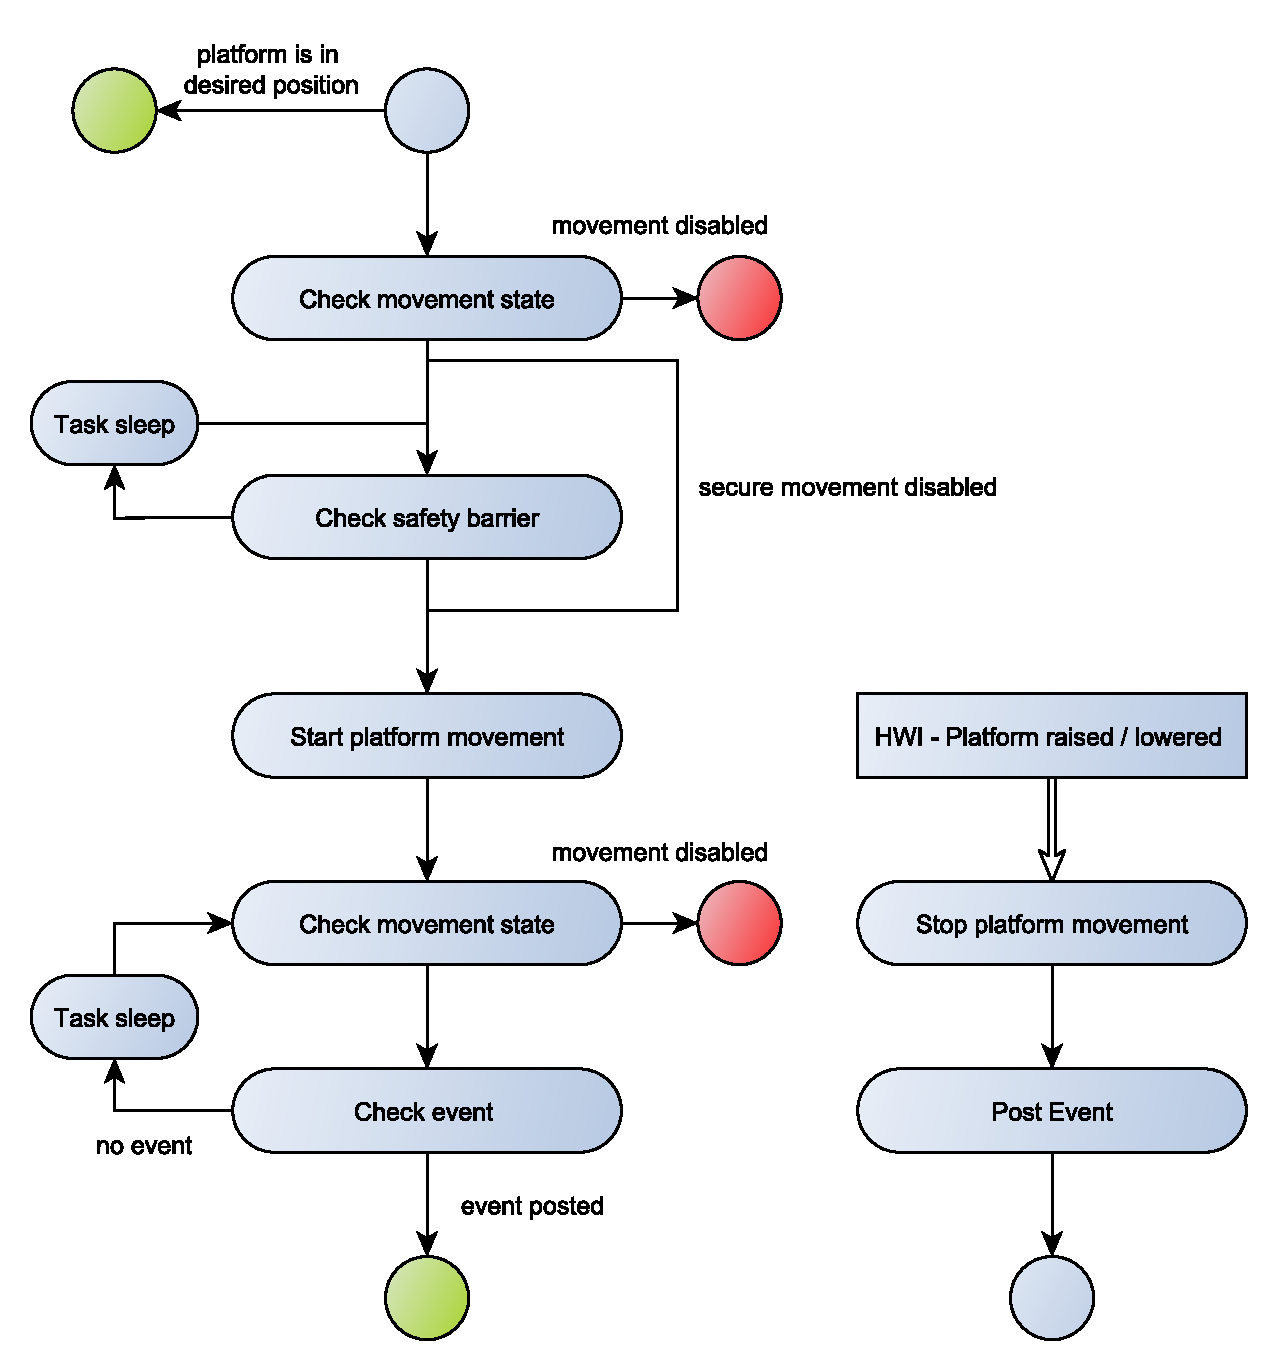
\includegraphics[width=0.8\textwidth]{media/Flow_Chart_MovePlatform.pdf} 	
		\caption{Flowchart - Move Platform}
		\label{fig:moveplatform}
	\end{center}
\end{figure}


% TODO: Table of measurements?

\section{User Interface} \label{sec:userinterface} %TODO: Pixel-Julian

In order to transfer data from the state machine to the display logic, a C struct called \texttt{festoData} is introduced. All the data that is needed to display is represented in that struct. Its internal representation is shown in listing \ref{struct}. Apart from the values of the current and the operating time, it includes the actual state of the screen as well as the measurements that are received during the automated processing of workpieces.

\begin{lstlisting}[label=struct, caption=festoData struct, style=customc]
typedef struct
{
	time_t 			theTime;
	uint32_t 		operatingTime;
	
	screenState_type 	screenState;
	thresholdState_type	thresholdState;
	calibrateState_type	calibrateState;
	
	material_type 		currentMaterial;
	color_type 		currentColor;
	uint32_t 		currentHeight;
	
	uint32_t		countTotal;
	uint32_t 		countAccepted;
	uint32_t 		countMetallic;
	uint32_t 		countBlack;
	
	uint32_t 		thresholdTop;
	uint32_t 		thresholdBottom;
	
	uint32_t 		calibrateFirst;
	uint32_t 		calibrateSecond;
	
	bool 			enableMovement;
	bool 			measuring;
} festoData_type;
\end{lstlisting}

These values are accessed and written by either the state machine or the button handler. No value is modified by both. 


The \texttt{updateScreenTask} is responsible for painting a new frame with updated values onto the screen.
It waits until the \texttt{Event\_Id\_06} is posted and then calls the corresponding drawing function.

This event itself is posted whenever the eventHandler adjusts the data that is part of the \texttt{festoData} struct.
This could for example be an adjustment of the current time or of the state of the screen.

There are three different screen states while each one of them is allowing the user to perform different actions. They are shown in figure \ref{fig:gui}.

\begin{figure} [H] 	
	\begin{center}
		\subfigure[Status]{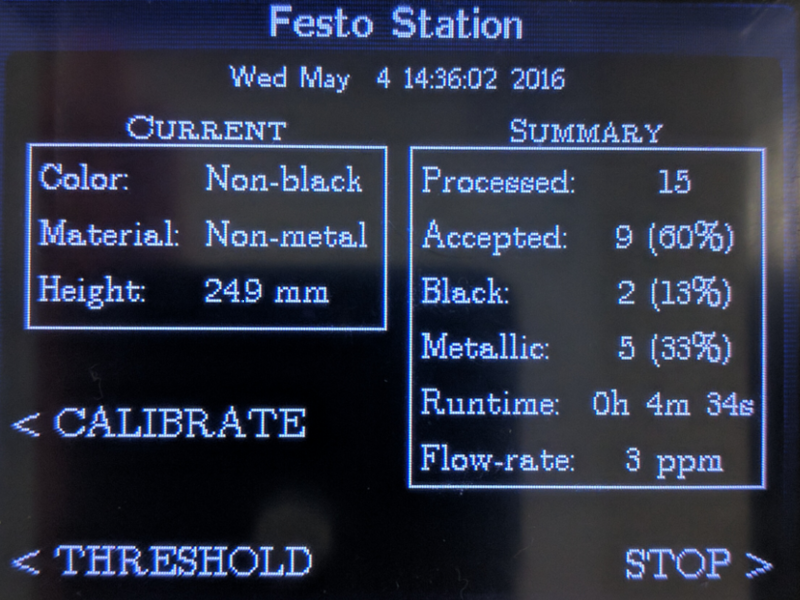
\includegraphics[width=0.30\textwidth]{media/Screenshot0.png}
			\label{fig:guiStatus}} 
		\quad
		\subfigure[Calibration]{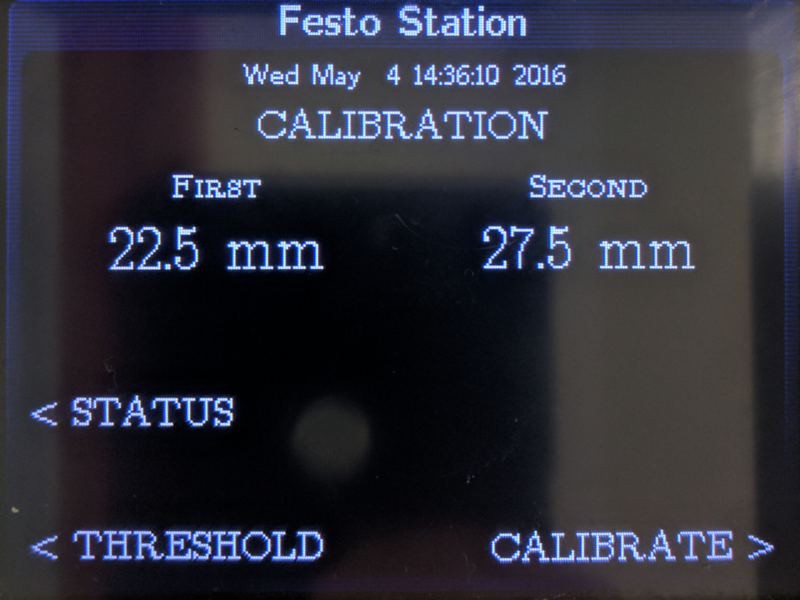
\includegraphics[width=0.30\textwidth]{media/Screenshot1.png}
			\label{fig:guiCalibrate}} 
		\quad
		\subfigure[Threshold]{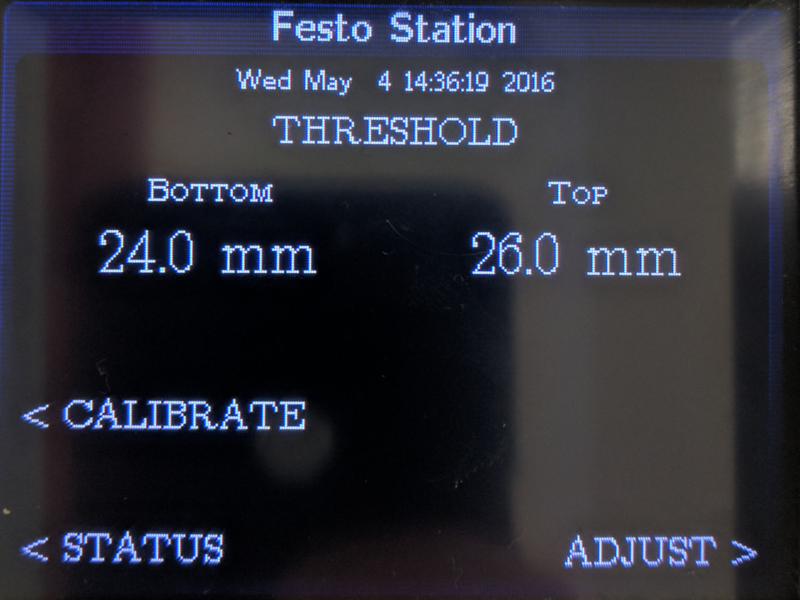
\includegraphics[width=0.30\textwidth]{media/Screenshot2.png}
			\label{fig:guiThreshold}} 
		\caption{GUI Screenshots}
		\label{fig:gui}
	\end{center}
\end{figure} 

The first display state shown in figure \ref{fig:guiStatus} is the status screen.
It shows all the values of the last measured workpiece and furthermore a summary of all the measured workpieces in total.
In addition, the total runtime and the current flow-rate are displayed.
While this screen is active, the two buttons on the left allow for %TODO: delete for?
 switching into another screen state, while the button on the right starts and stops the automation process of the measuring. %TODO: I would write testing instead of measuring

When the user goes into the calibration mode, the current values and the summary disappear and he is then asked to enter the height for the workpieces that will be used for calibration, as shown in figure \ref{fig:guiCalibrate}.
In this screen the buttons on the left are either used to switch again into another screen state or to adjust the calibration values.
The button on the right consecutively continues the calibration process.

Finally, the last screen state is the threshold mode.
As in the calibration mode, two values are displayed which can as well be adjusted by the user while using the buttons on the left.
The button on the right is again used for continuing and confirming.
All the workpieces that are measured in the automation process are compared against these values and will only be accepted if their height value is between these thresholds.

The drawing of the screen itself is done via the \texttt{updateScreen} function in the \texttt{screen.c} file.
At first the screen is cleared by painting a rectangle with the color of the background over the whole screen.
Afterwards a distinction of cases decides which screen is to be drawn.
With help of the functions \texttt{GrStringDraw} and \texttt{GrStringDrawCentered}  by the \textit{TivaWare™ Graphics Library} the strings will then be printed at the appropriate coordinates. 
Additionally the rectangles are drawn with the help of the \texttt{GrRectDraw} function.

%TODO: If possible please refer to the documents from the bibliography and add some section and keywords to the table.

\section{Calibration} %TODO: Timo

% Calibration necessary because values might change due to little changes of station
% Using two work pieces with specified height 
% Linear function (slope & y-intercept)
% ui workflow (up down to set height - select to measure)

% measured data 

The resistance probe of the testing station is providing a analogue output value. This output value gets converted by the ADC to a \textit{uint32\_t}-value. This value is proportional to the height of a work piece. 
It is necessary to determine the linear function that is describing the proportion between the measured value and the actual height of a work piece. Therefore a calibration routine is used.

The calibration gets triggered by a button press of the user in the corresponding view (See Sec. \ref{sec:userinterface}). The first thing to happen is that the state machine will jump into the \texttt{CALIBRATE\_SENSOR}-state after the event of the pressed button is received and will start the calibration routine (See Sec. \ref{sec:statemachine}). 

The procedure of this routine will be described in the following and is visualized in figure \ref{fig:calibration}: 
The platform will be moved to the lowered position. Afterwards it will be checked if the event was posted that indicates that the apply-button was pressed. In the meantime user is entering the actual height of the first work piece that is used for calibration and puts it onto the platform of the station. To trigger the measuring of the first piece the apply-button gets pressed that results in the posting of the corresponding event and to save the value (in $10^{-1}$mm) as \texttt{calibrateFirst} in the \texttt{festoData struct} (See. Sec. \ref{sec:userinterface}). 
After the event was detected the platform is moved to the raised position and the work piece gets measured and the value gets saved for later calculation.
The whole procedure gets repeated for the second work piece. \\
Once both work pieces were measured the slope and the y-intercept of the height function gets computed. Therefore it will be figured out which of the two entered work pieces is the taller one and then the following formulas are used:
\[slope = \frac{taller_{ref} - smaller_{ref}}{taller - smaller}\]
\[y\text{-}intercept = smaller_{ref} - (slope * smaller)\]
With the slope and y-intercept the actual height of work pieces can be computed in $10^{-1}$mm. This is done by the \texttt{getWorkpieceHeight(..)} of the driver library by entering the digital height sensor value in the formula (See. Sec. \ref{sec:driverlibrary}):
\[height = value * slope + y\text{-}intercept\]

\begin{figure}[H]
	\begin{center}
		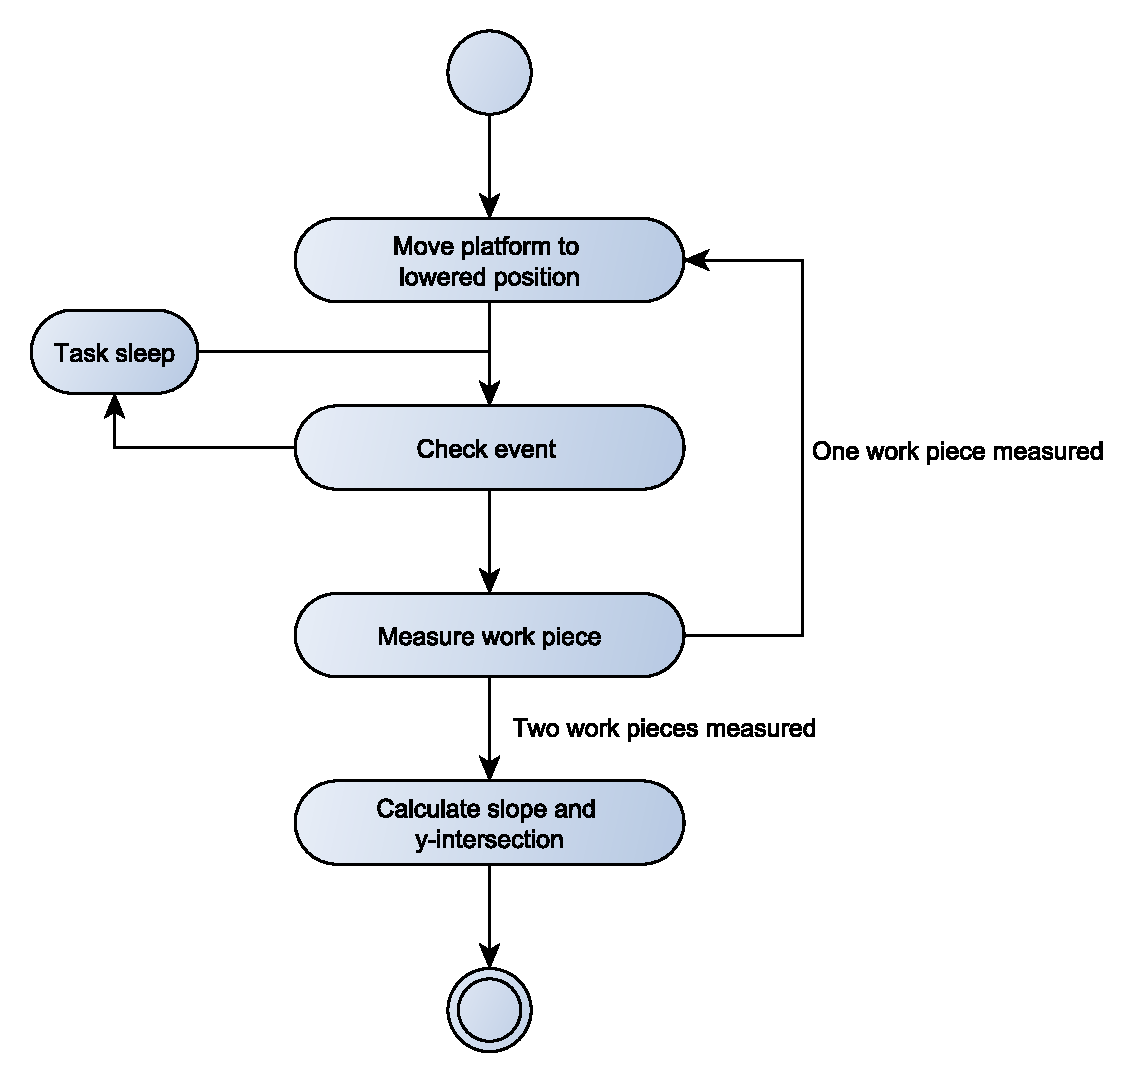
\includegraphics[width=0.7\textwidth]{media/Flow_Chart_Calibration.pdf} 	
		\caption{Flowchart - Height Sensor Calibration}
		\label{fig:calibration}
	\end{center}
\end{figure}

In addition to this a series of data was recorded to determine how precise the height sensor is and how accurate the output of the function is. 
